\documentclass{article}\usepackage[]{graphicx}\usepackage[]{color}
%% maxwidth is the original width if it is less than linewidth
%% otherwise use linewidth (to make sure the graphics do not exceed the margin)
\makeatletter
\def\maxwidth{ %
  \ifdim\Gin@nat@width>\linewidth
    \linewidth
  \else
    \Gin@nat@width
  \fi
}
\makeatother

\definecolor{fgcolor}{rgb}{0.345, 0.345, 0.345}
\newcommand{\hlnum}[1]{\textcolor[rgb]{0.686,0.059,0.569}{#1}}%
\newcommand{\hlstr}[1]{\textcolor[rgb]{0.192,0.494,0.8}{#1}}%
\newcommand{\hlcom}[1]{\textcolor[rgb]{0.678,0.584,0.686}{\textit{#1}}}%
\newcommand{\hlopt}[1]{\textcolor[rgb]{0,0,0}{#1}}%
\newcommand{\hlstd}[1]{\textcolor[rgb]{0.345,0.345,0.345}{#1}}%
\newcommand{\hlkwa}[1]{\textcolor[rgb]{0.161,0.373,0.58}{\textbf{#1}}}%
\newcommand{\hlkwb}[1]{\textcolor[rgb]{0.69,0.353,0.396}{#1}}%
\newcommand{\hlkwc}[1]{\textcolor[rgb]{0.333,0.667,0.333}{#1}}%
\newcommand{\hlkwd}[1]{\textcolor[rgb]{0.737,0.353,0.396}{\textbf{#1}}}%

\usepackage{framed}
\makeatletter
\newenvironment{kframe}{%
 \def\at@end@of@kframe{}%
 \ifinner\ifhmode%
  \def\at@end@of@kframe{\end{minipage}}%
  \begin{minipage}{\columnwidth}%
 \fi\fi%
 \def\FrameCommand##1{\hskip\@totalleftmargin \hskip-\fboxsep
 \colorbox{shadecolor}{##1}\hskip-\fboxsep
     % There is no \\@totalrightmargin, so:
     \hskip-\linewidth \hskip-\@totalleftmargin \hskip\columnwidth}%
 \MakeFramed {\advance\hsize-\width
   \@totalleftmargin\z@ \linewidth\hsize
   \@setminipage}}%
 {\par\unskip\endMakeFramed%
 \at@end@of@kframe}
\makeatother

\definecolor{shadecolor}{rgb}{.97, .97, .97}
\definecolor{messagecolor}{rgb}{0, 0, 0}
\definecolor{warningcolor}{rgb}{1, 0, 1}
\definecolor{errorcolor}{rgb}{1, 0, 0}
\newenvironment{knitrout}{}{} % an empty environment to be redefined in TeX

\usepackage{alltt}
\usepackage{amscd, amssymb, amsmath, verbatim, setspace}
\usepackage[left=1.0in, right=1.0in, top=1.0in, bottom=1.0in]{geometry}
\usepackage{mathrsfs}
\usepackage{listings}


\IfFileExists{upquote.sty}{\usepackage{upquote}}{}
\begin{document}

\begin{flushright}
Arif Ali\\
Math 640 Bayesian Statistics\\
April 21, 2016\\
\end{flushright}

\begin{center}
\LARGE\textbf{Homework \#5}
  \end{center}
  \section*{Exercise 1}
  \subsection*{Part A}
The posterior means can be calculated the following way.
\begin{knitrout}
\definecolor{shadecolor}{rgb}{1, 1, 1}\color{fgcolor}\begin{kframe}
\begin{verbatim}
set.seed(4231423)
library(MASS)
data(UScrime)
library(LearnBayes)

y = UScrime$y; n=length(y)
X = as.matrix(cbind(rep(1,n), UScrime[,-ncol(UScrime)]))

T = 1e4; k=dim(X)[2]; beta = matrix(NA, T, k)
g = n;  nu0 = 2;  s20 = 1

XtX.inv = solve(t(X)%*%X)
Sg = t(y)%*%(diag(1,n) - g/(g+1)*X%*%XtX.inv%*%t(X))%*%y
v = g/(g+1)*XtX.inv
m = v%*%t(X)%*%y

sigma2 = 1/rgamma(T, (nu0+n)/2, (nu0*s20+Sg)/2 )
for(t in 1:T) {
  beta[t,] = mvrnorm(1, m, sigma2[t]*v)
}

names(beta) = c("(Intercept)",names(UScrime)[-ncol(UScrime)])
Beta_means = apply(beta, 2, mean)
names(Beta_means) = c("(Intercept)",names(UScrime)[-ncol(UScrime)])
Beta_means
##   (Intercept)             M            So            Ed           Po1 
## -5854.0213914     8.6223843    -0.8114880    18.4902911    18.9415360 
##           Po2            LF           M.F           Pop            NW 
##   -10.8042356    -0.6578557     1.6918465    -0.7234731     0.4089468 
##            U1            U2           GDP          Ineq          Prob 
##    -5.6857842    16.3936888     0.9534558     6.9253094 -4780.8605899 
##          Time 
##    -3.4803122
\end{verbatim}
\end{kframe}
\end{knitrout}
The confidence intervals are
\begin{knitrout}
\definecolor{shadecolor}{rgb}{1, 1, 1}\color{fgcolor}\begin{kframe}
\begin{verbatim}
beta.ci = apply(beta, 2, quantile, c(0.025, 0.975))
colnames(beta.ci) = c("(Intercept)",names(UScrime)[-ncol(UScrime)])
t(beta.ci)
##                      2.5%        97.5%
## (Intercept) -9166.3045979 -2540.489511
## M               0.1356346    17.117501
## So           -304.4383476   303.383762
## Ed              5.7318849    31.062020
## Po1            -2.3172868    40.776414
## Po2           -34.9421674    12.459706
## LF             -3.5771120     2.346274
## M.F            -2.5033091     5.859471
## Pop            -3.3802632     1.876897
## NW             -0.9255687     1.725497
## U1            -14.4219511     3.126659
## U2             -1.1069140    33.359286
## GDP            -1.2410612     3.036100
## Ineq            2.2515701    11.566756
## Prob        -9514.3377455  -145.111528
## Time          -18.1444128    11.245169
\end{verbatim}
\end{kframe}
\end{knitrout}
The least square values for $\beta$ can be calculated using the lm function.
\begin{knitrout}
\definecolor{shadecolor}{rgb}{1, 1, 1}\color{fgcolor}\begin{kframe}
\begin{verbatim}
Crime.fit = lm(y~.,data= UScrime)
\end{verbatim}
\end{kframe}
\end{knitrout}
With respect the the differences between the Bayesian Method and the least square methods, we can determine the difference with the following.
\begin{knitrout}
\definecolor{shadecolor}{rgb}{1, 1, 1}\color{fgcolor}\begin{kframe}
\begin{verbatim}
Beta_means - Crime.fit$coefficients
##   (Intercept)             M            So            Ed           Po1 
## 130.266213115  -0.160633050   2.991962298  -0.342140358  -0.338897869 
##           Po2            LF           M.F           Pop            NW 
##   0.137956920   0.005970441  -0.048839080   0.009535018  -0.011499322 
##            U1            U2           GDP          Ineq          Prob 
##   0.141318531  -0.386278374  -0.008206634  -0.141900501  74.405225544 
##          Time 
##  -0.001294313
\end{verbatim}
\end{kframe}
\end{knitrout}
It's interesting to see that the difference between the posteior means and the values of $\beta$ calculated by the least squares method are very close. 
\begin{knitrout}
\definecolor{shadecolor}{rgb}{1, 1, 1}\color{fgcolor}\begin{kframe}
\begin{verbatim}
t(beta.ci) - confint(Crime.fit)
##                      2.5%        97.5%
## (Intercept) 138.960223850 122.82087598
## M            -0.139783539  -0.17311593
## So            2.753210816   3.79910375
## Ed           -0.437538765  -0.43341933
## Po1           0.043490411  -0.14523066
## Po2          -0.040273520  -0.55780301
## LF            0.084245856   0.01256842
## M.F          -0.092801085  -0.03240783
## Pop          -0.017189447  -0.02015995
## NW           -0.024228103  -0.01673541
## U1           -0.007907262   0.36682025
## U2           -1.094352421  -0.21320991
## GDP          -0.088440616  -0.03984540
## Ineq         -0.182574823  -0.13351934
## Prob        -24.533334845  75.61569183
## Time         -0.051719915   0.11051163
\end{verbatim}
\end{kframe}
\end{knitrout}
The difference between the Confidence Interval following the same pattern as with the means. That is attributed to the intercept and Prob; however, based on the values obtained, the differences aren't as significant.
\subsection*{Part B}
\begin{knitrout}
\definecolor{shadecolor}{rgb}{1, 1, 1}\color{fgcolor}\begin{kframe}
\begin{verbatim}
Problem1b = function(seed = F, graph = F){
  if(seed){
    set.seed(seed)
    }
  train = sample(nrow(UScrime), nrow(UScrime)*0.5)
  UScrime.train = UScrime[train,]
  UScrime.test = UScrime[-train,]
  Crimeb.fit = lm(y~.,data= UScrime.train)
  Crimeb.fit$coefficients
  Crimeb.fittedvalues = predict(Crimeb.fit, UScrime.test)

  y = UScrime.train$y; n=length(y)
  X = as.matrix(cbind(rep(1,n), UScrime.train[,-ncol(UScrime.train)]))

  T = 1e4; k=dim(X)[2]; beta = matrix(NA, T, k)
  g = n;  nu0 = 2;  s20 = 1

  XtX.inv = solve(t(X)%*%X)
  Sg = t(y)%*%(diag(1,n) - g/(g+1)*X%*%XtX.inv%*%t(X))%*%y
  v = g/(g+1)*XtX.inv
  m = v%*%t(X)%*%y

  sigma2 = 1/rgamma(T, (nu0+n)/2, (nu0*s20+Sg)/2 )
  for(t in 1:T) {
    beta[t,] = mvrnorm(1, m, sigma2[t]*v)
  }

  Beta_means = apply(beta, 2, mean)
  names(Beta_means) = c("(Intercept)",names(UScrime)[-ncol(UScrime)])
  Beta_means
  bayesian_predictions = (as.matrix(UScrime.test[,-ncol(UScrime.test)])%*%(Beta_means[-1])+Beta_means[1])[,1]
  
  mean((bayesian_predictions - UScrime.test$y)^2)
  
  if(graph){
    par(mfrow=c(1,2))
    plot(UScrime.test$y, Crimeb.fittedvalues, 
         main = "least-squares regression", 
         xlab = "observations", ylab = expression(hat(y[i])))
    plot(UScrime.test$y, bayesian_predictions, 
         main = "bayesian posterior means regression", 
         xlab = "observations", ylab = expression(hat(y[i])))
    
  }
  
  results = list(Crimeb.fit$coefficients, mean((Crimeb.fittedvalues-UScrime.test$y)^2),
                 Beta_means,mean((bayesian_predictions - UScrime.test$y)^2))
  names(results) = c("least-squares regression coefficients", "MSE", 
                     " posterior mean", "MSE posterior mean")
  return(results)
}

Problem1b(1e8, T)
\end{verbatim}
\end{kframe}
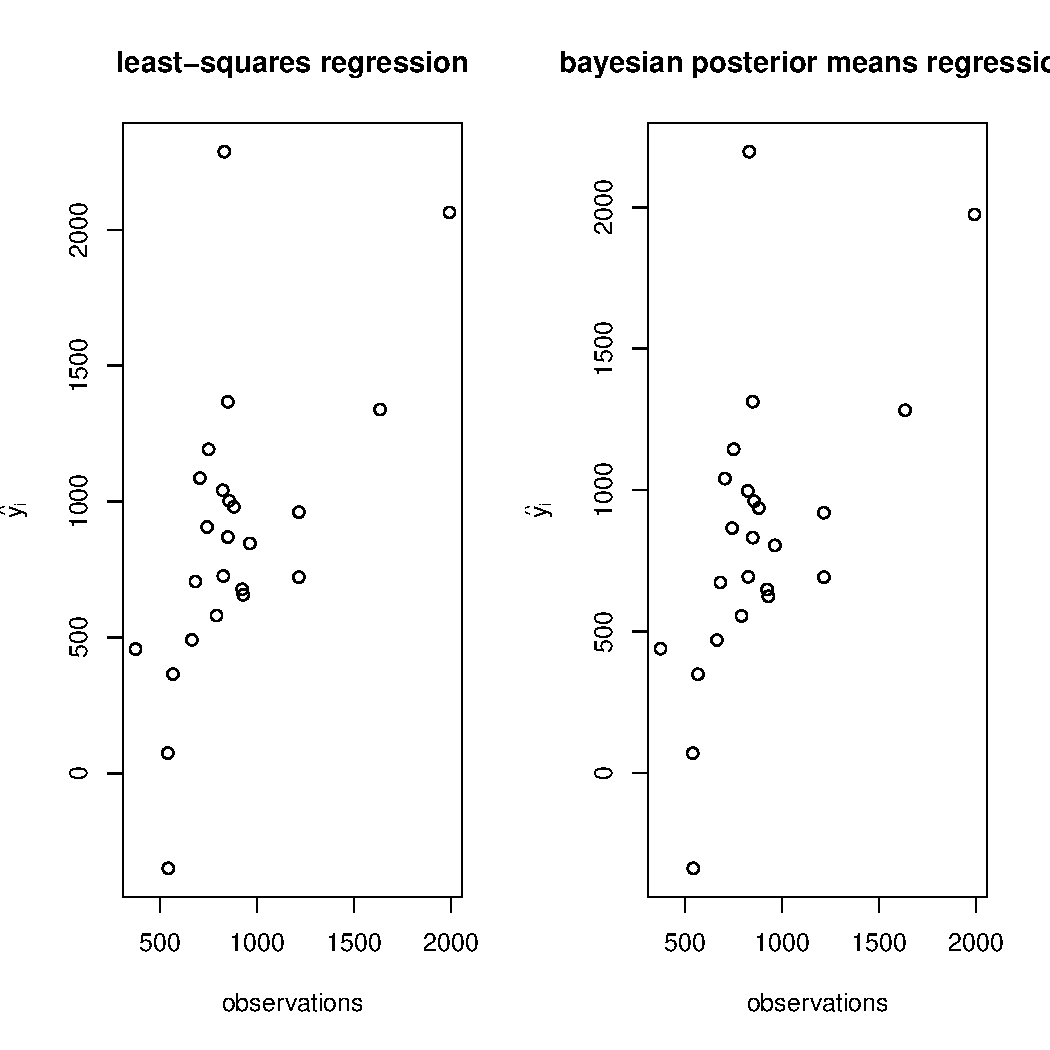
\includegraphics[width=1\linewidth]{figure/unnamed-chunk-7-1} 
\begin{kframe}\begin{verbatim}
## $`least-squares regression coefficients`
##   (Intercept)             M            So            Ed           Po1 
## -8.259814e+03  1.490893e+01  6.268855e+02  1.128908e+00 -1.292324e+01 
##           Po2            LF           M.F           Pop            NW 
##  2.694348e+01  8.477062e+00  1.030005e+00 -8.069709e-01  2.276716e-01 
##            U1            U2           GDP          Ineq          Prob 
##  1.929445e+00  1.392674e+01 -6.914113e-01 -2.167347e-01 -1.005828e+04 
##          Time 
##  5.982888e+00 
## 
## $MSE
## [1] 188881.3
## 
## $` posterior mean`
##   (Intercept)             M            So            Ed           Po1 
## -7948.3836292    14.3931292   598.8011211     1.0311238   -12.8756182 
##           Po2            LF           M.F           Pop            NW 
##    26.3771702     8.1412927     1.0008753    -0.7463585     0.2091552 
##            U1            U2           GDP          Ineq          Prob 
##     1.8268808    13.4431374    -0.6748428    -0.1946998 -9639.4103593 
##          Time 
##     5.7397735 
## 
## $`MSE posterior mean`
## [1] 176657.6
\end{verbatim}
\end{kframe}
\end{knitrout}
From the result, the method using the posterior mean performs better than one using the least squares estimates. 
\subsection*{Part C}
\begin{knitrout}
\definecolor{shadecolor}{rgb}{1, 1, 1}\color{fgcolor}\begin{kframe}
\begin{verbatim}
Problem1c = matrix(data = NA, nrow = 100, ncol = 2)
names(Problem1c) = c("least-squares regression MSE", "MSE  posterior mean")
for(i in 1:100){
  Problem1ci = Problem1b()
  Problem1c[i,]= c(Problem1ci[[2]], Problem1ci[[4]])
}
apply(Problem1c,2,mean, na.rm = T)
## [1] 173703.2 164701.3
\end{verbatim}
\end{kframe}
\end{knitrout}
\section*{Exercise 2}
\subsection*{Part A}
$logit(P(Y_{i}=1|\alpha,\beta,x_{i}))=log(P(Y_{i}=1|\alpha,\beta,x_{i}))-log(1-P(Y_{i}=1|\alpha,\beta,x_{i}))=\alpha+\beta*x_{i}\implies$

$\frac{(P(Y_{i}=1|\alpha,\beta,x_{i}))}{1-(P(Y_{i}=1|\alpha,\beta,x_{i}))}=exp(\alpha+\beta*x_{i})\implies$
$(P(Y_{i}=1|\alpha,\beta,x_{i}))=\frac{exp(\alpha+\beta*x_{i})}{1+exp(\alpha+\beta*x_{i})}$

$\therefore (P(Y_{i}=0|\alpha,\beta,x_{i})) = \frac{1}{1+exp(\alpha+\beta*x_{i})}$

$f(y_{i}|\alpha,\beta,x_{i})=\left(\frac{exp(\alpha+\beta*x_{i})}{1+exp(\alpha+\beta*x_{i})}\right)^{y_{i}}*\left(\frac{1}{1+exp(\alpha+\beta*x_{i})}\right)^{1-y_{i}}=$

$\left(\frac{exp(\alpha+\beta*x_{i})}{1+exp(\alpha+\beta*x_{i})}\right)^{y_{i}}*\left(1+exp(\alpha+\beta*x_{i})\right)^{y_{i}}\left(\frac{1}{1+exp(\alpha+\beta*x_{i})}\right)=\left(exp(\alpha+\beta*x_{i})\right)^{y_{i}}*\left(\frac{1}{1+exp(\alpha+\beta*x_{i})}\right)$

$\ensuremath{f(\boldsymbol{y}|\alpha,\beta,\boldsymbol{x})=\prod_{i=1}^{n}\left(exp(\alpha+\beta*x_{i})\right)^{y_{i}}*\left(\frac{1}{1+exp(\alpha+\beta*x_{i})}\right)=}$

$exp\left\{ log\left(\prod_{i=1}^{n}\left(exp(\alpha+\beta*x_{i})\right)^{y_{i}}*\left(\frac{1}{1+exp(\alpha+\beta*x_{i})}\right)\right)\right\} =$

$exp\left\{ \sum_{i=1}^{n}\left[log\left(exp(\alpha+\beta*x_{i})\right)^{y_{i}}-log\left(1+exp(\alpha+\beta*x_{i})\right)\right]\right\} =$

$exp\left\{ \sum_{i=1}^{n}\left[y_{i}*log\left(exp(\alpha+\beta*x_{i})\right)-log\left(1+exp(\alpha+\beta*x_{i})\right)\right]\right\}$
\subsection*{Part B}
$r=\frac{p(\theta^{*}|\boldsymbol{y},\boldsymbol{x})}{{p(\theta^{t-1}|\boldsymbol{y},\boldsymbol{x})}}=$

$=\frac{p(\boldsymbol{y}|\theta^{*},\boldsymbol{x})*p(\theta^{*})}{p(\boldsymbol{y}|\theta^{t-1},\boldsymbol{x})*p(\theta^{t-1})}=$

$\frac{exp\left\{ \sum_{i=1}^{n}\left[y_{i}*log\left(exp(\alpha^{*}+\beta^{*}*x_{i})\right)-log\left(1+exp(\alpha^{*}+\beta^{*}*x_{i})\right)\right]\right\} }{exp\left\{ \sum_{i=1}^{n}\left[y_{i}*log\left(exp(\alpha^{t-1}+\beta^{t-1}*x_{i})\right)-log\left(1+exp(\alpha^{t-1}+\beta^{t-1}*x_{i})\right)\right]\right\} }*\frac{p(\alpha^{*})*p(\beta^{*})}{p(\alpha^{t-1})*p(\beta^{t-1})}$

\begin{knitrout}
\definecolor{shadecolor}{rgb}{1, 1, 1}\color{fgcolor}\begin{kframe}
\begin{verbatim}
library(MASS)
msparrownest <- read.table("~/Documents/Georgetown/Bayesian-Statistics-Mathematics-640/HW5/msparrownest.dat", quote="\"", comment.char="")
names(msparrownest) = c("nests", "wingspan")
y = msparrownest$nests; n=length(y)
x = msparrownest$wingspan
X = as.matrix(cbind(rep(1,n), msparrownest[,"wingspan"]))
proposal_var = n*mean(y)*(1-mean(y))*solve(t(X)%*%X)

ratio = function(thetastar, theta_pre){
  return(exp(sum(y*log(exp(thetastar[1]+thetastar[2]*x))-
            log(1+exp(thetastar[1]+thetastar[2]*x))))/
    (exp(sum(y*log(exp(theta_pre[1]+theta_pre[2]*x))-
               log(1+exp(theta_pre[1]+theta_pre[2]*x)))))*
      dnorm(thetastar[1], 0,10)*dnorm(thetastar[2],0,10)/
      (dnorm(theta_pre[1], 0,10)*dnorm(theta_pre[2],0,10)))
}
  

T = 1e5
theta = matrix(nrow=T, ncol=2)
theta[1,] = c(0,0)
accept = rep(0,T)

for(t in 2:T){
  theta_star = mvrnorm(1,theta[t-1,], Sigma = proposal_var)
  r = ratio(theta_star, theta[t-1,])
  u = runif(1)
  if(u<r){
    theta[t,] = theta_star
    accept[t] = 1
  } else{
    theta[t,] = theta[t-1,]
  }
}
par(mfrow = c(1,2))
plot(theta[,1], type = 'l', xlab = "t", ylab = expression(alpha))
plot(theta[,2], type = 'l', xlab = "t",ylab = expression(beta))
\end{verbatim}
\end{kframe}
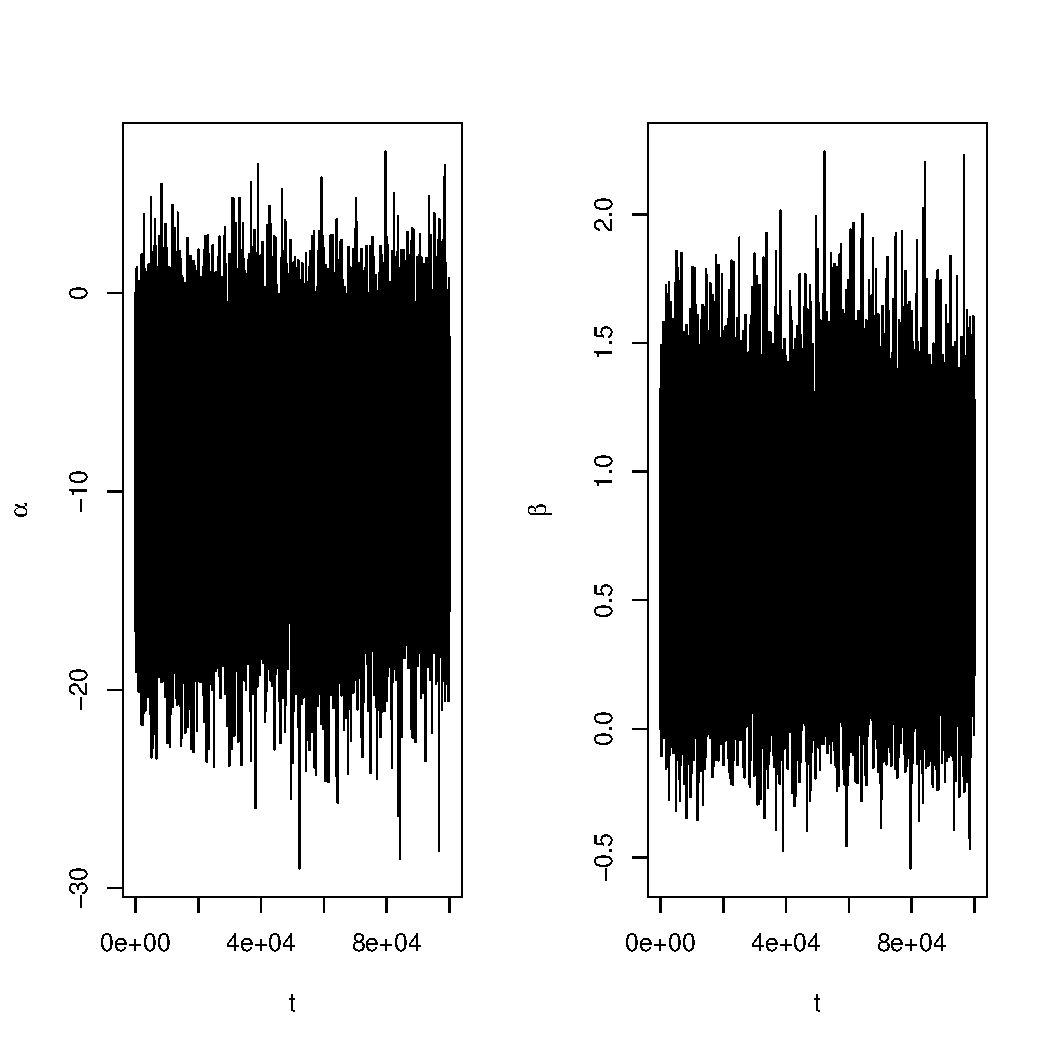
\includegraphics[width=1\linewidth]{figure/unnamed-chunk-9-1} 

\end{knitrout}
Based on trace the trace plots, there does not seem to be a failure of convergence to the stationary distribution for either $\alpha$ or $\beta$.
\begin{knitrout}
\definecolor{shadecolor}{rgb}{1, 1, 1}\color{fgcolor}\begin{kframe}
\begin{verbatim}
nburn = 1e3
mean(accept[-(1:nburn)])
## [1] 0.3978182
\end{verbatim}
\end{kframe}
\end{knitrout}
The acceptance rate is approximately 39.6\%.
\begin{knitrout}
\definecolor{shadecolor}{rgb}{1, 1, 1}\color{fgcolor}\begin{kframe}
\begin{verbatim}
library(coda)
theta.mcmc = as.mcmc(theta[-(1:nburn),])
effectiveSize(theta.mcmc)
##     var1     var2 
## 12584.82 12448.95
\end{verbatim}
\end{kframe}
\end{knitrout}
Based on the effectiveSize, $>1000$ for both $\alpha$ and $\beta$ have been obtained.
\subsection*{Part C}
\begin{knitrout}
\definecolor{shadecolor}{rgb}{1, 1, 1}\color{fgcolor}\begin{kframe}
\begin{verbatim}
# The posterior estimates for alpha and beta.
apply(theta, 2, mean)
## [1] -8.7142122  0.6939065
hist(theta[,1], probability = TRUE,
     main = expression(alpha), xlim = c(-30,30))
lines(density(theta[,1]), col = "blue")
curve(dnorm(x, 0,10), add = TRUE, col = "red")
legend("topleft", legend = c("posterior density", "prior density"), 
       fill = c("blue", "red"))
\end{verbatim}
\end{kframe}
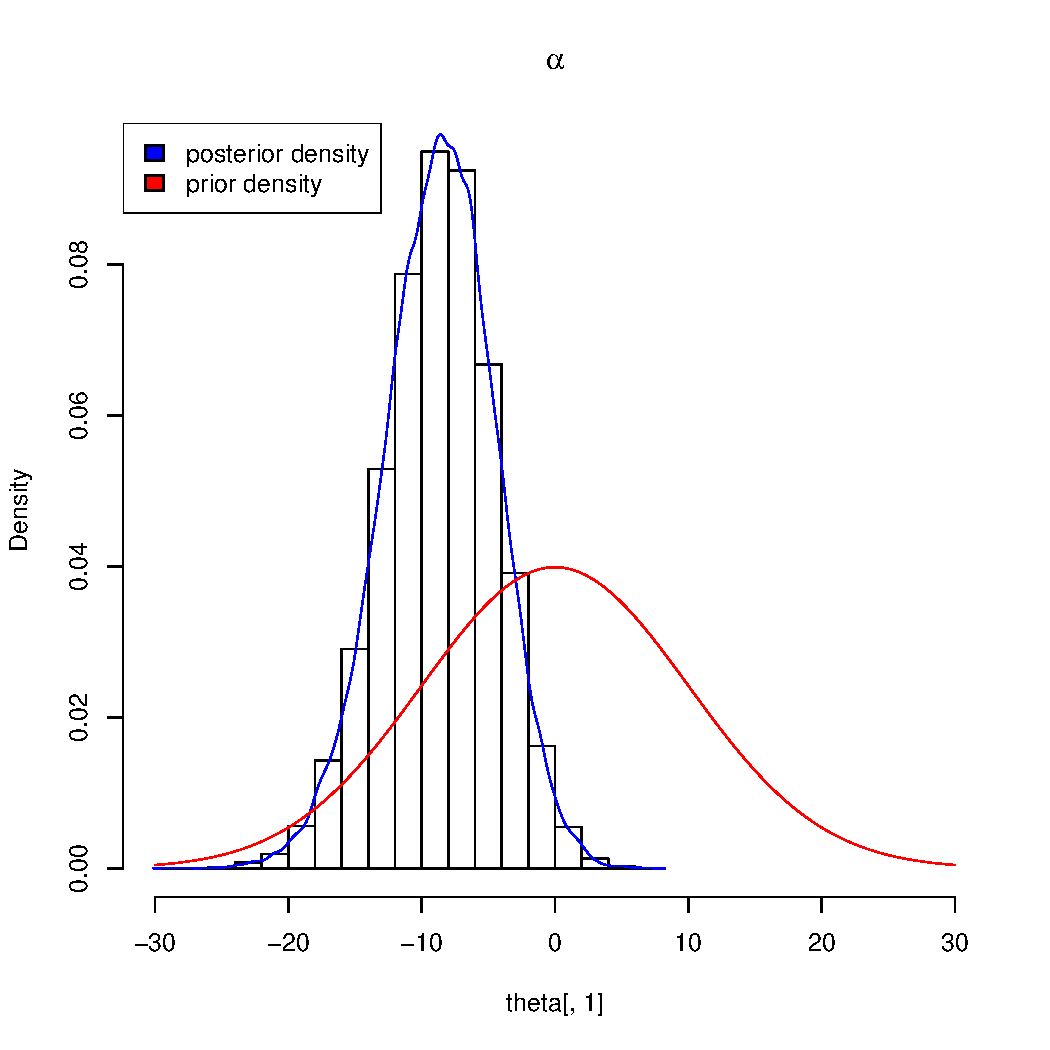
\includegraphics[width=1\linewidth]{figure/unnamed-chunk-12-1} 
\begin{kframe}\begin{verbatim}
hist(theta[,2], probability = TRUE, 
     main = expression(beta), xlim = c(-30,30))
lines(density(theta[,2]), col = "blue")
curve(dnorm(x, 0,10), add = TRUE, col = "red")
legend("topleft", legend = c("posterior density", "prior density"), 
       fill = c("blue", "red"))
\end{verbatim}
\end{kframe}
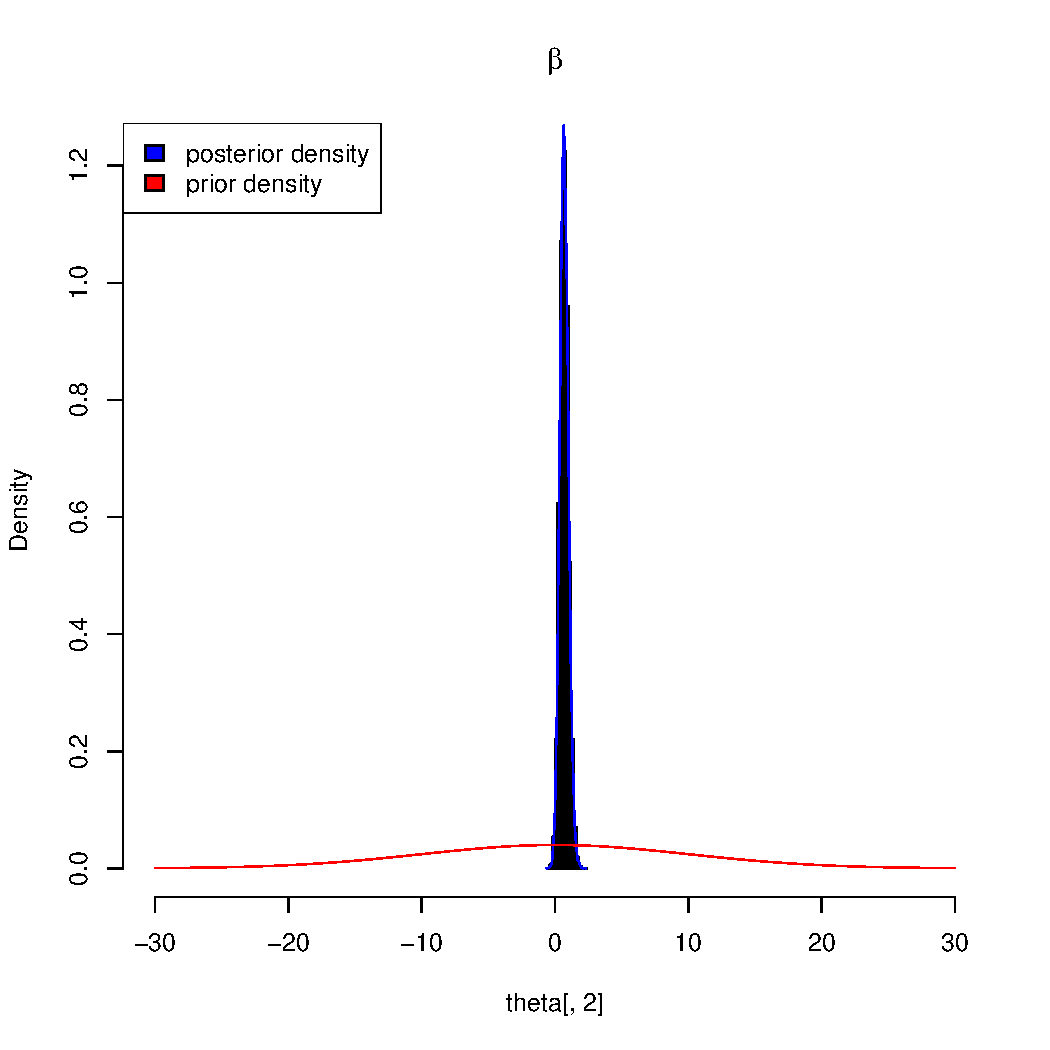
\includegraphics[width=1\linewidth]{figure/unnamed-chunk-12-2} 

\end{knitrout}
The prior estimates for both $\alpha$ and $\beta$ are 0 because the densities for are defined as $N(0,10^{2})$. The difference between the posterior and prior estimate for $\alpha$ is approximately 8.63 where as the difference between those of beta are approximately 0.69. 
For the different in the posterior and prior densities for alpha, there is a shift to the left (hence the negative mean) and a lower standard deviation. For beta, the change in SD is much more significant. 
\subsection*{Part D}
\begin{knitrout}
\definecolor{shadecolor}{rgb}{1, 1, 1}\color{fgcolor}\begin{kframe}
\begin{verbatim}
fab = function(x,theta){
  return(exp(theta[1]+theta[2]*x)/(1+exp(theta[1]+theta[2]*x)))
}
confidence_band = matrix(nrow = length(x), ncol = 3)

confidence_band[,1] = x
for(i in 1:length(x)){
  fabresults = rep(0, nrow(theta))
  for(t in 1:nrow(theta)){
  fabresults[t] = fab(x[i], theta[t,])
  }
  confidence_band[i, 2:3] = quantile(fabresults, c(0.025,0.975))
  }
confidence_band = as.data.frame(confidence_band)
names(confidence_band) = c("x_i", "lower", "upper")
confidence_band = confidence_band[order(confidence_band$x_i),]
plot(nests~wingspan, data = msparrownest, pch =20, 
     ylab = expression(f[ab](x)))
lines(upper~x_i, data = confidence_band, col = "red")
lines(lower~x_i, data = confidence_band, col = "red")
\end{verbatim}
\end{kframe}
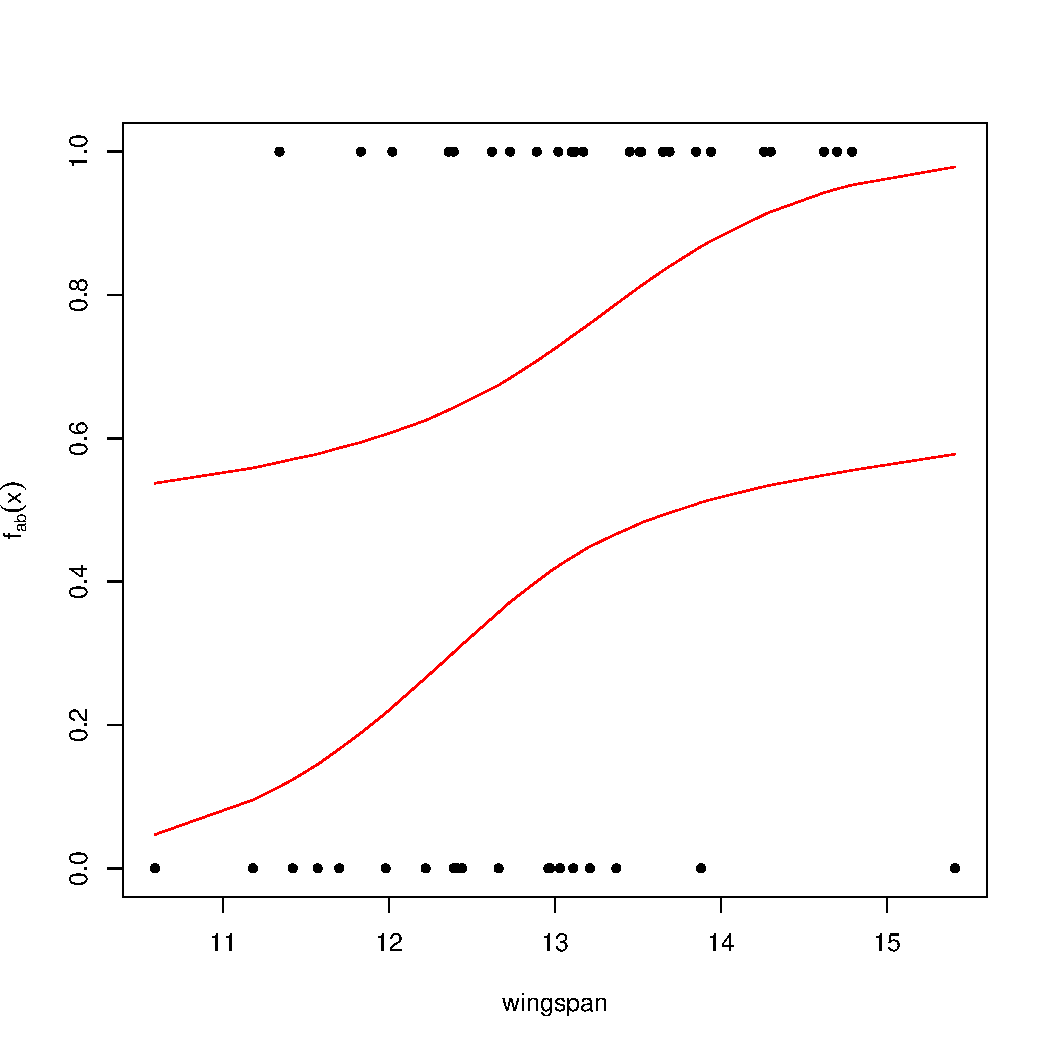
\includegraphics[width=1\linewidth]{figure/unnamed-chunk-13-1} 

\end{knitrout}
\end{document}
